
\chapter{Interface homme machine}

\section{Fonctionnalités de l' IHM}

L'interface homme-machine est un des composant essentiel de notre projet. En effet, c'est grâce à elle que l'utilisateur va pouvoir juger de la qualité du logiciel. Ainsi, conformément au  cahier des charges, on va retrouver les fonctionnalités suivantes :


\section{Ergonomie}

\begin{figure}[h]
 \centering
 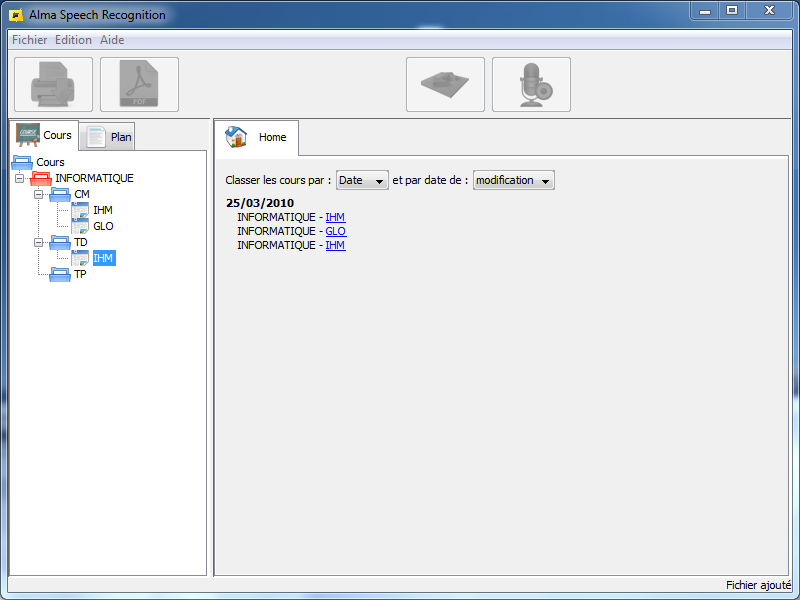
\includegraphics[scale=0.6]{./images/homePanel.png}
 % homePanel.png: 0x0 pixel, -2147483648dpi, 0.00x0.00 cm, bb=
 \caption{IHM - Panneau d'accueil}
 \label{fig:homePanel}
\end{figure}



\begin{figure}[h]
 \centering
 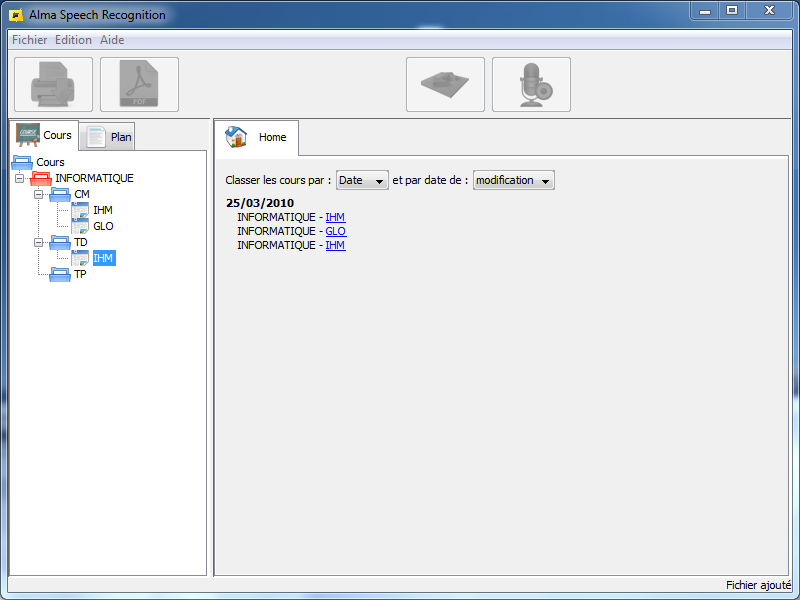
\includegraphics[scale=0.6]{./images/homePanel.png}
 % homePanel.png: 0x0 pixel, -2147483648dpi, 0.00x0.00 cm, bb=
 \caption{IHM - Panneau de travail}
 \label{fig:homePanel}
\end{figure}
